\section{Thermodynamik der feuchten Luft}
\label{sec:Thermodynamik der feuchten Luft}

Ein Verdampfer hat die Aufgabe einer Umgebung Energie in Form von Wärme zu entziehen. Hierfür wird in einem Wärmeübetrager flüssiges Kältemittel verdampft. Das verdampfende Kältemittel kühlt zunächst den Wärmeübertrager, danach wird über die Wärmeübertrager-Lamellen der vorbeiströmende Luft Wärme entzogen. 

Bei dem Kühlprozess durch einen Verdampfer kommt es zwischen dem Wärmeübertrager und der feuchten Luft verschiedenen thermodynamischen Phänomenen. Die auftretenden Phänomene lassen sich in folgende Gruppen einordnen:

\begin{itemize}
\item	Abkühlung der feuchter Luft 
\item 	Wassertropfenbildung auf Lamellenoberfläche 
\item	Kristallbildung auf Lamellenoberfläche.
\end{itemize}

In den nachfolgenden Abschnitten \ref{subsec:Feuchte Luft} und \ref{subsec:Reifbildung} werden die Phänomene kurz erklärt.

\subsection{Feuchte Luft}
\label{subsec:Feuchte Luft}

\begin{figure}[htb]
\centering		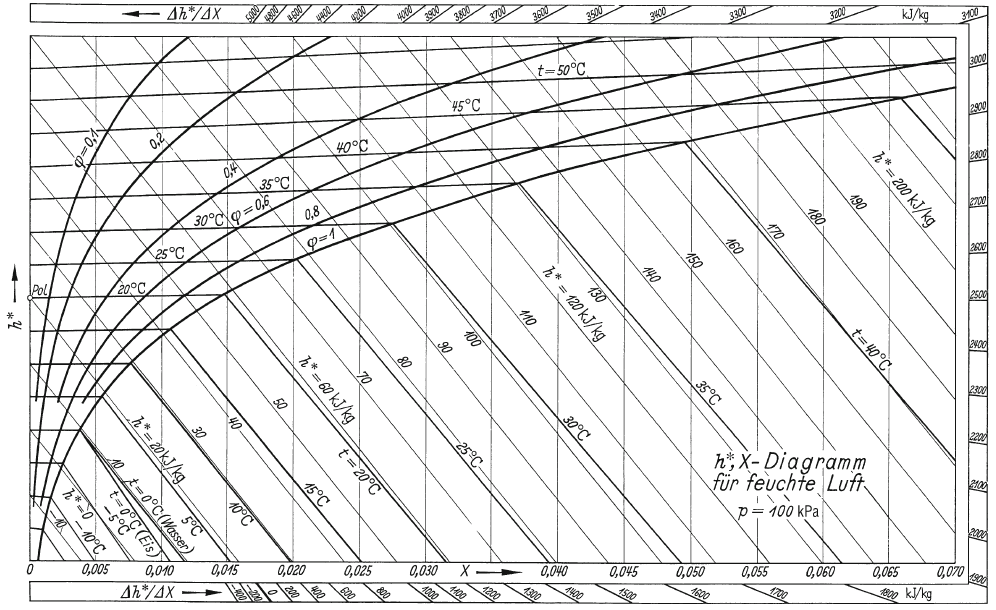
\includegraphics[width=0.85\textwidth]{Pictures/h_x_Diagramm_Beahr.png}
\caption{$h^*$, $X$- Diagramm für feuchte Luft bei einem Gesamtdruck $p= $ 100 kPa \citep{Baehr2013}}
\label{fig:h_x_diagramm}
\end{figure}


Bei dem Wärmeentzug durch den Verdampfer wird  zunächst die noch nicht gesättigte feuchte Luft abgekühlt. Luft besitzt die Eigenschaft eine bestimmte Menge Wasser aufnehmen zu können. Warme Luft kann mehr Wasser aufnehmen als kalte Luft. Das Verhältnis von der aufgenommene Masse Wasser zur Masse Luft ist definiert als Beladung: 

\begin{equation}
X = \frac{m_W}{m_L}.
\label{eq:Beladung}
\end{equation}

In dieser Formel bezieht sich $m_W$ auf gasförmige, flüssige oder feste Form von Wasser und $m_L$ auf die Masse der trockenen Luft.  $X$ kann werden zwischen 0 für trockene Luft und $\infty$ für reines Wasser annehmen. In der Regel bleibt $X$ jedoch kleiner als 0,1. 

Die absolute Feuchte ist definiert als das Verhältnis von Masse des Wasserdampfers $m_W$ zum eingenommen Volumen $V$ der feuchten Luft. Die Formel lautet: 

\begin{equation}
\varrho := \frac{m_W}{V} = \frac{p_w}{R_W T}.
\label{eq:Absolute Feuchte}
\end{equation}


Die relativen Feuchte $\varphi$ ist das Verhältnis der absoluten Feuchte im Verhälnis zur Maximalwert oder Sättigungswert der absoluten Feuchte: 

\begin{equation}
 \varphi := \frac{\varrho}{\varrho_W^s}.
 \label{eq:Rel Feuchte}
\end{equation}

Wird nun in die Gleichung \ref{eq:Beladung} die relative Feuchte aus Gleichung \ref{eq:Rel Feuchte} eingesetzt, ergibt sich eine weitere Formel für die Beladung $X$. 

\begin{equation}
X = \frac{m_W}{m_L} = 0,622 \frac{p_{W}^s}{p/\varphi - p_{W}^s}.
\label{eq:Beladung 2}
\end{equation}

Hierbei ist $p_{W}^s$ der Partialdruck des Sättigungspunktes.
Betrachtet man nur die Wasserdampfbeladung der Luft, so lässt sich feststellen, dass die maximale Menge an aufzunehmenden Wasser einen Grenzwert hat. Dieser Grenzwert wird Sättigungswert der Wasserdampfbeladung genannt und ist eine Funktion abhängig von der Temperatur und dem Druck.  Sie berechnet sich nach dem Gesetz von Dalton zu :

\begin{equation}
 X_s (T,p) = 0,622 \frac{p_{W}^s}{p - p_{W}^s}.
 \label{eq:Sättigungsbeladung}
\end{equation}

Bei der Abkühlung von feuchter Luft kann der Fall eintreten, dass $X > X_s$ ist. Sprich die Beladung der trockenen Luft ist größer als das alles im Wasserdampf aufgenommen werden kann. Der erste Tropfen Kondensat bildet sich und Wasser fällt aus. Es ergibt sich eine Kondesationsmenge von:

\begin{equation}
\Delta X m_L = (X - X_s)m_L.
\label{eq:Delta_X}
\end{equation}

Die Wassermenge $X_s m_L$ ist gasförmig von der trockenen Luft gespeichert. Die Kondensationsmenge $\Delta X m_L$ setzt sich nun an Keimpunkten in der Umgebung ab oder wird als Nebel aus der Gasphase ausgeschieden. Keimzellen für Wassertropfen können zum Beispiel Verunreinigungen oder raue Oberflächen sein. Das höchste treibende Potential für eine solche Keimzelle hat der kälteste Punkt im System. In unserem Anwendungsfall ist das der Wärmeübertrager des Verdampfer. Da der Verdampfer zur Bereitstellung der Kälteleistung und einer funktionierenden Wärmeübertragung stets eine Temperaturdifferenz zwischen dem Kältemittel und der vorbei strömenden Luft  bereitstellt,  bilden sich hier die ersten Tropfen. Je nach ursprünglicher Beladung der Luft bilden sich die Tropfen eher am Anfang oder Ende des Wärmeübertrager. War die feuchte Luft schon vor dem Eintritt in den Wärmeübertrager bereits stark gesättigt, bilden sich Tropfen am Eingang der Lamellen. 
\citep{Baehr2013}


\subsection{Reif- und Eisbildung}
\label{subsec:Reifbildung}

Liegt die Oberflächentemperatur auf dem Wärmeübertrager des Verdampfers nicht nur unter dem Taupunktpunkt der feuchten Luft sondern auch unter dem Gefrierpunkt, kann es zum Gefrieren der kondensierten Tropfen und/oder zur Desublimation von Wasserpartikel auf der Oberfläche kommen. Dieser Abschnitt soll einen Überblick über diese zwei thermodynamischen Phänome geben. Da in dieser Arbeit nicht der Reifbildungsprozess im Hauptfokus steht, sondern  der technische Aspekt der Abtauung, wird der Eisbildungsprozess hier nur kurz erläutert.

In der Literatur gibt es zahlreiche Quellen, die sich mit der Reif- bzw. Eisbildung auseinander setzen. Die Quellen beschreiben den Kristallbildungsprozess sowohl aus der rein theoretisch Sicht als auch simulationsrelevanten und technischen Überlegungen und Untersuchungen. Der scheinbar triviale Prozess von der Bildung eines Eiskristalles auf einer Oberfläche und sein weiteres Wachstumsverhalten ist sehr komplex und Gegenstand zahlreicher aktueller und schon abgeschlossener Forschungsprojekten.

Neben den theoretischen Grundlagen wird in der Arbeit von \textsc{\citeauthor{Schydlo2010}} ein Simulationsmodell für den Reifbildungs- und Abtauprozess auf einem Rohr entwickelt. Zudem sind bisherigen Arbeiten zu der Thematik in \citep{Schydlo2010} aufgelistet und zusammengefasst. 
Praktische Untersuchungen sowie Versuchsaufbauten zum Thema der Vereisung von Luftkühler werden in \textsc{\citeauthor{Sahinagic2004}} und \textsc{\citeauthor{Kosowski2009}} beschrieben. In den Arbeiten wurden die Vereisungs- und innovative Abtauungsprozesse von einer CO$_2$-Wärmepumpe, die zur Heizung von Passivhäuser eingesetzt wird, untersucht.   



Es gibt zahlreiche Einflussgrößen die auf den Prozess und die Form des Eiskristalls und späteren Reif einwirkten. 
  Die wichtigsten Einflussgrößen sind die Luftgeschwindigkeit, die Lufttemperatur, die Luftfeuchte, die Oberflächentemperatur und die Zeit. Um eine den Reif charakterisieren zu können, werden folgende Größen zur Hilfe genommen die Reifdicke, die Reifdichte, die Porösität und die Wärmeleitfähigkeit. 

In der Arbeit von \textsc{\citeauthor{Hayashi1977}} aus dem Jahre 1977 wird der Eiskristallwachstum in drei Phasen unterteilt:

\begin{enumerate}
\item Eindimensionales Kristallwachstum
\item Reifschichtwachstumsphase 
\item Vergletscherung.
\end{enumerate}


\begin{figure}[htb]
\centering		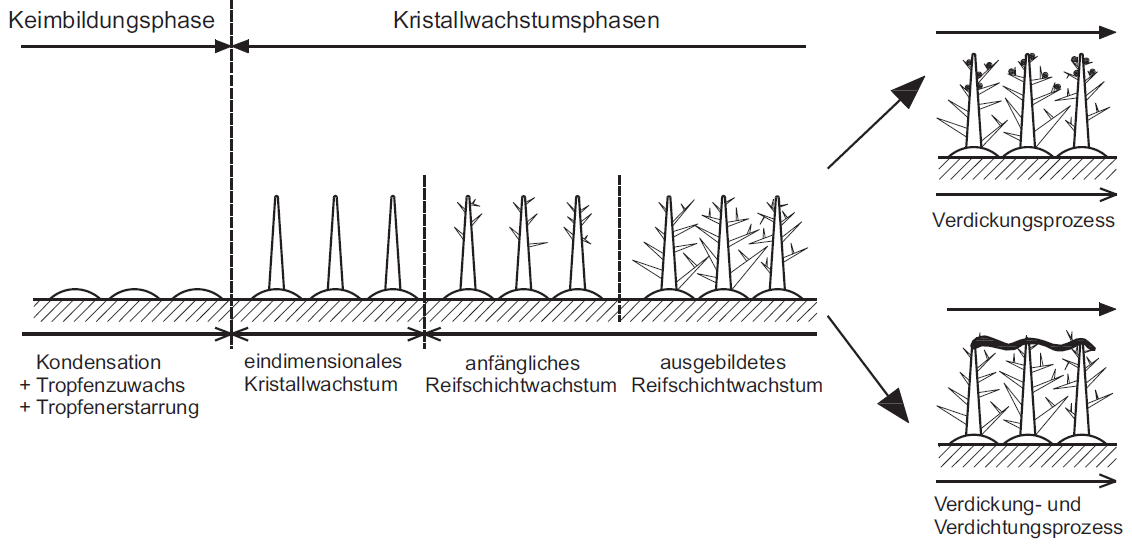
\includegraphics[width=0.85\textwidth]{Pictures/Reifbildungsphasen_Schydlo.png}
\caption{Kristallwachstum auf einer ebenen Oberfläche \citep{Schydlo2010}}
\label{fig:Kristallwachstum}
\end{figure}


In Abbildung \ref{fig:Kristallwachstum} sind die drei Kristallwachstums-Phasen nach \textsc{\citeauthor{Hayashi1977}} sowie die vorhergehende Keimbildungsphase, , eingeführt in \citep{Sahinagic2004}, dargestellt. 

\subsection*{Keimbildungsphase}

In der Keimbildungsphase bilden sich zunächst Wassertropfen auf der Lamellenoberfläche, die trotz Temperaturen kleiner als der Gefrierpunkt nicht erstarren, sondern wachsen zu größeren Tropfen an. Je kleiner die Unterkühlung desto größer werden die Tropfen bevor sie erstarren und in die erste Kristallwachstumsphase übergehen. 

\subsection*{Eindimensionales Kristallwachstum}
Die erste Phase ist gekennzeichnet durch Kristallwachstum senkrecht zur Oberfläche und mit einheitlicher Wachstumsgeschwindigkeit. Dies führt zu einer erhöhten Rauigkeit aufgrund der sich stetig vermehrenden Kristalle. 

\subsection*{Reifschichtwachstumsphase}
In der zweiten Phase beginnt das dreidimensionale Wachstum. Die Kristalle fangen an sich miteinander zu verästeln. Ein poröses Kristallgitter entsteht. Aufgrund des  Wärmeleitwiderstandes, der mit der Reifdicke steigt, erhöht sich die Oberflächentemperatur der Reifschicht. Desweiteren kommt es zu einem Massenstrom innerhalb der Reifschicht, ausgelöst durch Diffusion. Die Diffusion rührt aus  den  Konzentrationsunterschiede zwischen der Lamelle und der Reifoberfläche. Der Wassermassenstrom läuft in das poröse Kristallgitter und gefriert dort in Nähe der Lamelle. Die Dichte der Reifschicht steigt und mit ihr der Wärmewiderstand. Dies führt zu einer Erhöhung der Oberflächentemperatur der Reifschicht und schließlich zur Überschreitung des Gefrierpunktes von Eis. Die Spitzen des Kristalle schmelzen und es bildet sich Kondensat. Die dritte Wachstumsphase beginnt. 

\subsection*{Vergletscherung}

Das flüssige Wasser läuft aufgrund der Kapillarwirkung der Kristalle in die Zwischenräume des Kristalgitters und gefriert dort wieder. Die Kristallgitter werden dichter und kompakter. Dies führt zur Steigerung der Wärmeleitfähigkeit der Reifschicht. Es wird von einer Vergletscherung gesprochen. Die Oberflächentemperatur der Reifschicht sinkt erneut und fällt erneut unter den Gefrierpunkt. Nun kann die feuchte Luft erneut an der Oberfläche des Reifs desublimieren. Der Prozess wiederholt sich solange bis das Eis so kompakt ist, dass kein weiteres Kondensat mehr in die Reifschicht eindringen kann. 
    



